
\documentclass[12pt,a4paper,final]{article}
\usepackage[utf8]{inputenc}
\usepackage[francais]{babel}
\usepackage[T1]{fontenc}
\usepackage{amsmath}
\usepackage{amsfonts}
\usepackage{amsthm}
\usepackage{color}
\usepackage{amssymb}
\usepackage{graphicx}
\usepackage{algorithm}
\usepackage{algorithmic}
\usepackage{fancyhdr}
\usepackage[fs]{umons-coverpage}


%%###### START CHANGE HERE ######
\author{S. Opsommer \& R. Cambier}
\title{Rapport du projet Pac-Man}
\umonsAuthor{\begin{tabular}{lll}
\textsc{Cambier} & Robin & ROBIN.CAMBIERR@student.umons.ac.be\\
\textsc{Opsommer} & Sophie & SOPHIE.OPSOMMER@student.umons.ac.be\\
\end{tabular} }
%% The main title of your thesis
\umonsTitle{Rapport du projet Pac-Man}
%% The sub-title of your thesis
\umonsSubtitle{Projet réalisé dans le cadre \\de la 1ère Master en Sciences Informatiques \\pour le cours de \og Software Evolution \fg}
%% Your supervisor(s)
\umonsSupervisor{\begin{tabular}{ll}
\textit{Titulaire} : & T. \textsc{Mens} \\
\textit{Assistant} : & M. \textsc{Claes} \\
\end{tabular}}
%% The date (or academic year)
\umonsDate {\hfill Ann\'ee Acad\'emique 2014-2015}
%%###### END CHANGEMENT ######

\newcommand{\smalltitle}[1]{\bigskip\large\textbf{#1}\par\normalsize\medskip}
\newcommand{\partitle}[1]{\bigskip\textit{\underline{#1}}\par\medskip}
\newcommand{\annexe}[1]{figure~\ref{#1} (page~\pageref{#1})}

\newtheorem{defi}{Définition}
\newtheorem{note}{Note}
\newtheorem{prop}{Propriété}
\newtheorem{exemple}{Exemple}
\newtheorem{corollaire}{Corollaire}
\newtheorem{lemme}{Lemme}
\newtheorem{rem}{Remarque}
\newtheorem{thm}{Théorème}

\fancyhf{}
\chead{\leftmark}
\rfoot{\thepage}

\begin{document}

\umonsCoverPage
\pagebreak

\pagestyle{fancy}

\thispagestyle{empty}
\newpage
\tableofcontents
\newpage

%%###### LE RAPPORT COMMENCE ICI ######
\thispagestyle{empty}
%\smalltitle{......}
\vspace*{\stretch{1}}
\begin{abstract}
\addcontentsline{toc}{section}{Résumé}
Ce \emph{rapport} est rendu dans le cadre du cursus de première année de \og Master en Sciences Informatiques\fg  pour le cours de \emph{Software Evolution} (dont le titulaire est Mr. \emph{T. Mens} et l'assistant est Mr. \emph{M. Claes} en année académique 2014-2015) . Le but de ce rapport est de présenter les résultats de la réalisation du projet Pac-Man.
\end{abstract}
\vspace*{\stretch{1}}

\newpage
\section{Introduction}\label{sec:intro}
\subsection{Problème posé}
A partir d'un code existant, ce projet consiste à : 
\begin{itemize}
\item analyser la qualité du logiciel, en utilisant des techniques d'analyse statique du code (par exemple, la détection du code dupliqué et des bad smells, les diverses métriques de qualité) et les outils d'analyse dynamique du code (par exemple, le profilage, la couverture du code et des tests);
\item améliorer la qualité et la structure du code (en utilisant des refactorings, en introduisant des design patterns, et en modularisant le code) ;
\item étendre le logiciel avec de nouvelles fonctionnalités (évolution), et étudier l'effet de cela sur la qualité du code;
\item tester le logiciel avant et après chaque modification. Ceci implique que vous devez ajouter des tests unitaires (unit tests) pour au moins les fragments du code modifiés ou ajoutés, et d'appliquer des tests de régression à chaque modification.
\end{itemize}

\subsection{Etapes clés}
Les étapes clés du projet sont les suivantes : (chronologiquement)
\begin{enumerate}
\item Analyse de la qualité de la premiére version du code (section \ref{etape1})
\item Ajout de tests unitaires à la première version du code (section ...), et vérification de la couverture des tests
\item Refactoring du code pour en améliorer la qualité et la structure (section ...)
\item Analyse des améliorations de qualité et tests de régression (section ...)
\item Extension du logiciel et ajout des tests unitaires pour cette extension (section ...)
\item Analyse de la qualité de cette extension et tests de régression (section ...)
\item Etude de l'historique de la qualité logicielle entre toutes les versions du code (section ...)
\end{enumerate}
%%%%%%%%%%%%%%%%%%%%%%%%%%%%%%%%%%%%%%%%%%%%%%%%%%%%%%%%%%%%%%%%%%%%%%%%%%%%%%%%%%
\section{Etape 1 : Première analyse de la qualité du logiciel }\label{sec:etape1}
\subsection{Enoncé}
Le but de la première étape clé est d'analyser la qualité du logiciel pour avoir une première idée de ce qu'il faudra corriger si l'on désire améliorer la qualité. Cette première analyse est également l'occasion de comprendre l'architecture et la dynamique du système.
Pour cette étape clé il est demandons de :
\begin{enumerate}
\item Calculer la valeur de plusieurs métriques logicielles permettant d'estimer la qualité du logiciel, d'interpréter les résultats des métriques, et de mettre en évidence les modules (packages, classes ou méthodes) qui devraient être traités prioritairement afin d'améliorer leur qualité ainsi que la raison pour laquelle ils sont prioritaires.
\item Déterminer les classes et les méthodes qui sont couvertes par des tests unitaires, et mettre en évidence les méthodes pour lesquelles de nouveaux tests unitaires devraient être créés prioritairement.
\item Répertorier les portions de code qui ne sont pas utilisées et qui pourraient donc être supprimées sans altérer le comportement du système.
\item Répertorier les portions de code qui sont redondantes (code dupliqué) et qui pourraient donc être éliminées par une restructuration du système sans altérer son comportement.
\item Détecter la présence de bad smells. En trouvez-vous une plus forte concentration dans certains modules ?
\item Analyser les performances du système en terme d'utilisation CPU et de consommation de mémoire. Repérez les parties du code créant un goulot d'étranglement et précisez les modules qui devraient être retravaillés afin de procéder à un déoulottage du système.
\end{enumerate}
Décrivez la qualité globale du système. Quel serait, selon vous, le coût nécessaire à sa maintenance et à son évolution ?
\subsection{Résultat}

Voici le tableau des résultats de l'analyse des différentes métriques : 
\begin{tabular}{|l|l|}
\hline
Métrique & Outil utilisé + Résultat \\ & Interprétation des résultats \\ & Modules à traiter prioritairement + justification\\
\hline
\multicolumn{2}{|c|}{Techniques d'analyse statique du code} \\
\hline
Code dupliqué & CodePro Tools -> Find Similar Code : 10 blocs de \\
& code (visible sur la \annexe{SimilarCode} et les suivantes)\\
& sont semblable. \\
& Ce résultat n'est pas alarmant mais mérite d'être\\
& refactoré. \\
& Les classes Tile.java, GameTest.java,  \\
& ButtonPanel.java, MainUITest.java, MapParser.java, \\
&  PacmanKeyListener.java,PacmanKeyListener.java, \\
&  PacmanKeyListener.java, GameTest.java,Board \\
& sont à traiter puique c'est elle qui contiennent du \\
& code dupliqué. \\
\hline
Respect des & \\
conventions de codage & \\
\hline
Dépendences cycliques & \\
\hline
Performances & \\
\hline
Structure du code & \\
\hline
Style du code & \\
\hline
Design flaws  & \\
\hline
Antipattern  & \\
\hline
Test & \\
\hline
Dataflow  & \\
\hline
Documentation & \\
\hline
\multicolumn{2}{|c|}{Outils d'analyse dynamique du code} \\
\hline
Profilage & \\
\hline
Couverture du code & \\
\hline
Tests & \\
\hline
\end{tabular}

NB : 
- slide 4 : outils

Images : 
- $Métrique_0.png$
- 

%%%%%%%%%%%%%%%%%%%%%%%%%%%%%%%%%%%%%%%%%%%%%%%%%%%%%%%%%%%%%%%%%%%%%%%%%%%%%%%%%%
\section{Etape 2 : Ajout de tests unitaires}\label{sec:etape2}
\subsection{Enoncé}
Votre première analyse a révélé la présence de certains problèmes de qualité du code de l'application.
Avant d'envisager la correction de ces problèmes, il faut s'assurer que les modifications que vous apporterez au code source ne modifieront pas le comportement du logiciel.
Etendez et complétez le jeu de tests unitaires fourni avec le code source afin de vous prémunir d'une telle modification. Effectuez également une analyse de couverture de tests.
Quelle garantie avez-vous que vos futures modifications ne pourront pas casser le système ?

\subsection{Résultat}



%%%%%%%%%%%%%%%%%%%%%%%%%%%%%%%%%%%%%%%%%%%%%%%%%%%%%%%%%%%%%%%%%%%%%%%%%%%%%%%%%%
\section{Etape 3 : Refactoring en vue d'améliorer la qualité}\label{sec:etape3}
\subsection{Enoncé}
Avec les tests unitaires ajoutés dans l'étape précédente, vous pouvez vérifier automatiquement (jusqu'à un certain point) la préservation du comportement du logiciel. Réalisez les modifications nécessaires à l'amélioration de la qualité et la structure du logiciel. 
Vos ressources et votre temps étant limités, commencez par établir les modifications devant être réalisées en priorité. Sur base de quels critères réalisez-vous cette priorisation ?
Refactorisez progressivement votre code, en vous assurant systématiquement que tous les tests déjà présents s'exécutent avec succès. Souvenez-vous que vos modifications doivent améliorer la qualité du code, et non étendre ou modifier le comportement du logiciel.

\subsection{Résultat}



%%%%%%%%%%%%%%%%%%%%%%%%%%%%%%%%%%%%%%%%%%%%%%%%%%%%%%%%%%%%%%%%%%%%%%%%%%%%%%%%%%
\section{Etape 4 : Analyse de la qualité du logiciel}\label{sec:etape4}
\subsection{Enoncé}
Réalisez une étude similaire à celle décrite en Section ... La qualité du logiciel s'est-elle améliorée ? Les problèmes les plus critiques ont-ils été résolus ? Au vu de cette seconde analyse, quels sont les points qui devraient à présent être améliorés ?
\subsection{Résultat}



%%%%%%%%%%%%%%%%%%%%%%%%%%%%%%%%%%%%%%%%%%%%%%%%%%%%%%%%%%%%%%%%%%%%%%%%%%%%%%%%%%
\section{Etape 5 : Extensions}\label{sec:etape5}
\subsection{Enoncé} 
Il vous est demandé d'étendre le logiciel afin d'y ajouter certaines fonctionnalités ou d'en améliorer la qualité. Chaque équipe doit réaliser au moins deux extensions diférentes, décrites dans la section ... .
Utilisez un processus de développement dirigé par les tests (test-driven development) : lors du développement des extensions, ajoutez de nouveaux tests unitaires pour tester le comportement prévu de l'extension. Effectuez également des tests de régression avec les tests unitaires déjà présents, afin de vous assurer que le comportement initial n'a pas été modifié.
\subsection{Résultat}



%%%%%%%%%%%%%%%%%%%%%%%%%%%%%%%%%%%%%%%%%%%%%%%%%%%%%%%%%%%%%%%%%%%%%%%%%%%%%%%%%%
\section{Etape 6 : Analyse de la qualité du logiciel}\label{sec:etape6}
\subsection{Enoncé} 
Pour chaque extension ajoutée, réalisez une analyse de qualité similaire à celle décrite en Section ... Au vu de cette analyse, quels sont les points qui devraient à présent être améliorés ?
\subsection{Résultat}



%%%%%%%%%%%%%%%%%%%%%%%%%%%%%%%%%%%%%%%%%%%%%%%%%%%%%%%%%%%%%%%%%%%%%%%%%%%%%%%%%%
\section{Etape 7 : Analyse de l'évolution de la qualité logicielle}\label{sec:etape7}
\subsection{Enoncé} 
Analysez l'évolution de la qualité du logiciel entre les diférentes versions, en utilisant les résultats d'analyse de qualité des sections ..., ... et ... . Montrez cette évolution graphiquement et interprètez-la.
\subsection{Résultat}







%%%%%%%%%%%%%%%%%%%%%%%%%%%%%%%%%%%%%%%%%%%%%%%%%%%%%%%%%%%%%%%%%%%%%%%%%%%%%%%%%%
Quelque exemple d'utilisation. \textit{"Un peu d'italique"} \textbf{Du Gras}. Pour séparer deux paragraphe il suffit de mettre deux enter (une ligne blanche en gros)

Et voila un nouveau paragraphe :)\\
On peut egalement simplement revenir en arriere comme ca \\

Une petite liste a puce ? numéroté?

\begin{itemize}
\item $V$ est un ensemble fini de noeuds
\item $E$ est un ensemble d'arcs reliant deux noeuds
\end{itemize}

\begin{enumerate}
\item Remplacer la valeur de la racine par celle du dernier noeud, celui qui sera le plus à droite de la dernière ligne (le "1" dans l'exemple de la figure~\ref{heapExample}(a)).
\item Supprimer ce dernier noeud
\item Faire redescendre tant que nécessaire la nouvelle racine.
\end{enumerate}
Une image ? Avec une reference dans un texte ? no probleme :p

Un graphe orienté est défini par un couple: $G=(V,E)$.
La figure~\ref{graphExample} illustre un graphe.

La complexité c'est pas un simple O(lg n) mais $\mathcal{O}(\log_2 n)$.\\

\smalltitle{un petit titre qui n'apparait pas dans la table des matiere}
blablabla

\partitle{encore un plus petit titre}
blablabla

Un algorithme ? ouille ouille ouille :p mais on si habitue. Le caption sera le titre visible et le label sera ce que tu devra utiliser pour le referencer comme ca Alogo~\ref{extractMin}

%\begin{algorithm}[H]
%\caption{extractMin($A$)}\label{extractMin}
%\begin{algorithmic}[1]
%\STATE $min\gets A[1]$
%\STATE $A[1]\gets A[A.heapsize]$
%\STATE $A.heapsize\gets A.heapsize - 1$
%\STATE heapify($A, 1$)
%\end{algorithmic}
%\end{algorithm}

%\begin{algorithm}[H]
%\caption{heapify($A,i$)}\label{heapify}
%\begin{algorithmic}[1]
%\STATE $l\gets $left($i$)
%\STATE $r\gets $right($i$)
%\IF{$l \leq A.heapsize$ \AND $A[l] < A[i]$ }
%\STATE $smallest\gets l$
%\ELSE
%\STATE $smallest\gets i$
%\ENDIF
%\IF{$r <leq A.heapsize$ \AND $A[r] < A[smallest]$}
%\STATE $smallest\gets r$
%\ENDIF
%\IF{$i \neq smallest$}
%\STATE switch($A[i], A[smallest]$)
%\STATE heapify($A, smallest$)
%\ENDIF
%\end{algorithmic}
%\end{algorithm}

%\begin{algorithm}[H]
%\caption{decreaseKey($A,i,key$)}\label{heapify}
%\begin{algorithmic}[1]
%\IF{$key > A[i]$}
%\STATE \textbf{error} "la nouvelle clé doit être inférieur à la valeur actuel"
%\ENDIF
%\STATE $A[i]\gets key$
%\WHILE{$i>1$ \AND $A[$parent($i$)$] > A[i]$}
%\STATE switch($A[i],A[$parent($i$)$]$)
%\STATE $i\gets $parent($i$)
%\ENDWHILE
%\end{algorithmic}
%\end{algorithm}

Des theorme, lemme, propriete ? sa marche aussi :). De nouveaux tu peux reference le label :) Lemme~\ref{upper-bound_prop}

\begin{lemme}[Propriété de borne supérieur]\label{upper-bound_prop}
Nous avons à tout moment $v.d \geq \delta(s,v) \forall v \in V$, et une fois que $v.d$ atteins $\delta(s,v)$ il ne changera plus.
\end{lemme}

\begin{corollaire}[Propriété d'absence de chemin]\label{no_path_prop}
Si il n'existe pas de chemin allant de $s$ à $v$ alors nous avons à tout moment $v.d = \delta(s,v) = \infty$.
\end{corollaire}

\begin{prop}[Propriété de convergence]\label{convergence_prop}
Si $s \leadsto u \rightarrow v$ est un plus court chemin dans $G$ pour $u, v \in V$ donné et si $u.d = \delta(s,u)$ avant que l'arc ($u,v$) ne soit relaxé alors $v.d = \delta(s,v)$ après la relaxation.
\end{prop}

\begin{thm}[Thm de convergence]\label{convergence_thm}
Si $s \leadsto u \rightarrow v$ est un plus court chemin dans $G$ pour $u, v \in V$ donné et si $u.d = \delta(s,u)$ avant que l'arc ($u,v$) ne soit relaxé alors $v.d = \delta(s,v)$ après la relaxation.
\end{thm}

des symbole grec, mathematique $\delta(a), \sigma(a), \neq, \leq, \geq, ...$\\
Ca doit etre entre dollard. Pareil pour toutes les variables, formule, ...\\
on n'ecrit pas l'index i mais l'index $i$

\newpage
\section{Annexes} \label{sec:annexe}
\appendix %permet de changer la numérotation en lettre
\section{Annexe : 1}\label{SimilarCode}
Dans cette section se trouve les différentes annexes qui permettent d'identifier les blocs de dode dupliqués détecté par CodePro. La première image répertorie les 10 blocs. De la seconde à l'avant dernière, les images illustres les blocs de code. La dernière image illustres les 6 derniers blocs de code et est issue du rapport généré par CodePro parce que Eclipse les masque.
\begin{figure}
	\centering
	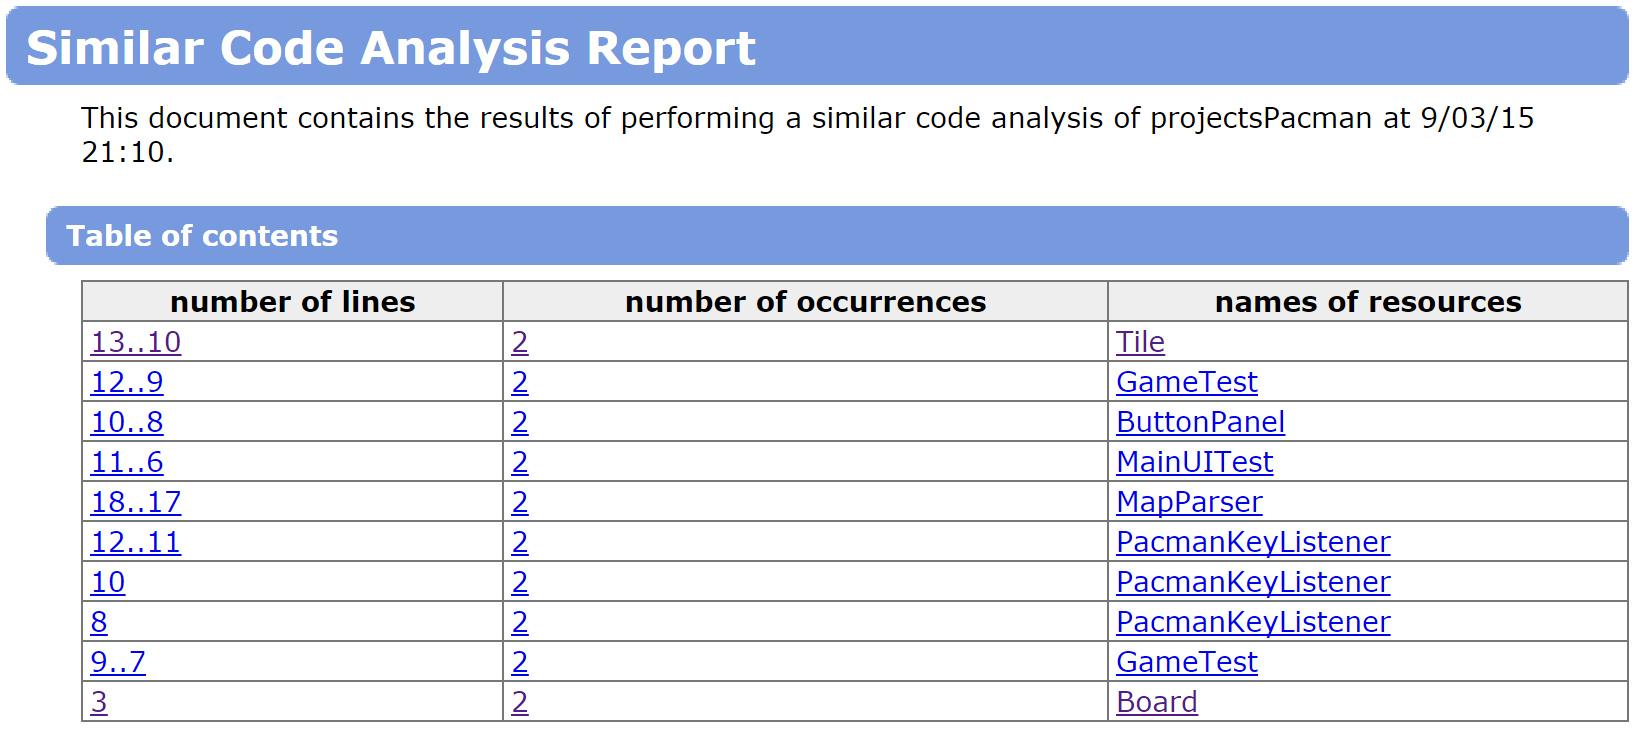
\includegraphics[width=\textwidth]{images/SimilarCode_00.png}
	\caption{\label{SimilarCode0}Résultat de l'analyse de code redondant par CodePro}
\end{figure}
\begin{figure}
	\centering
	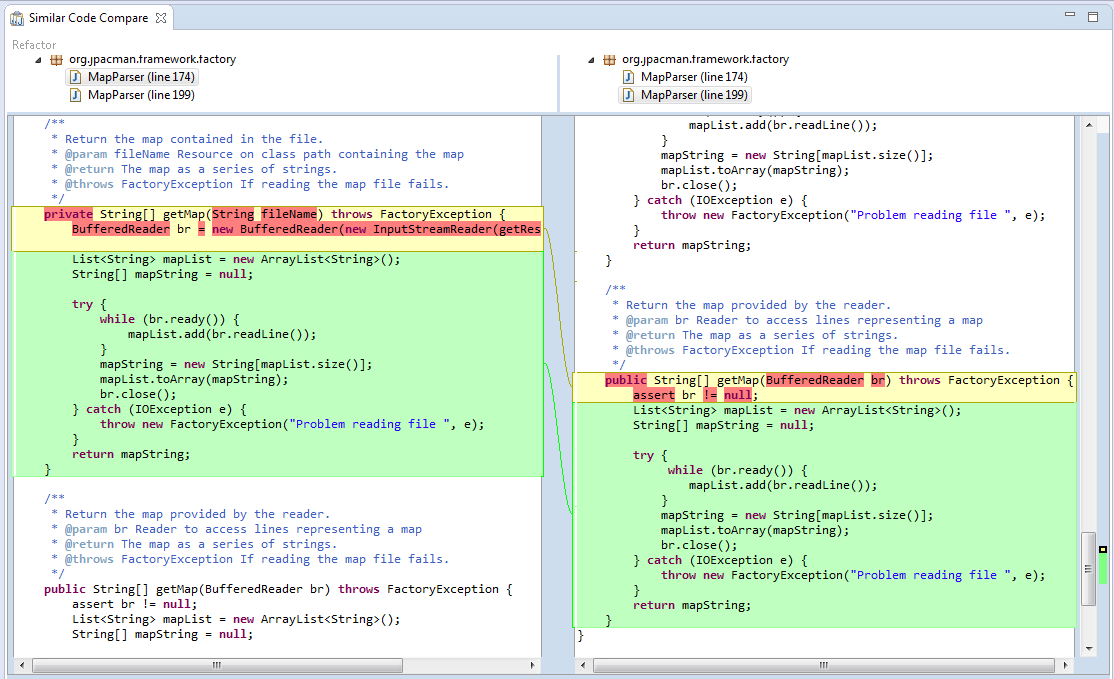
\includegraphics[width=\textwidth]{images/SimilarCode_1.png}
	\caption{\label{SimilarCode1}Détail de l'analyse de code redondant par CodePro}
\end{figure}

\begin{figure}
	\centering
	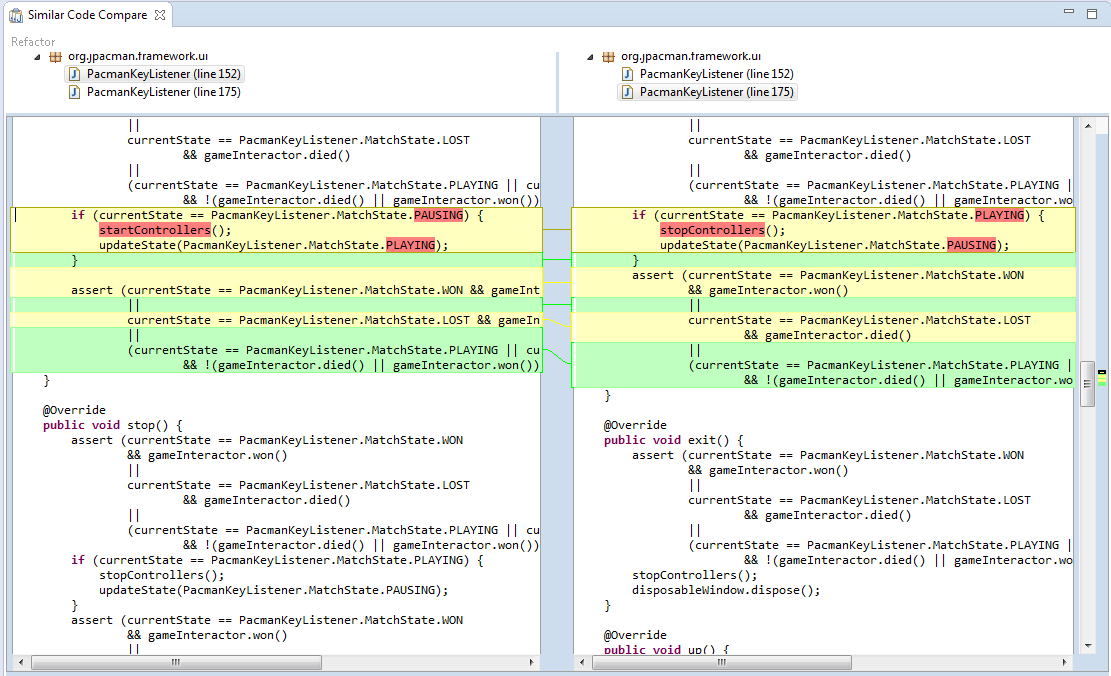
\includegraphics[width=\textwidth]{images/SimilarCode_2.png}
	\caption{\label{SimilarCode2}Détail de l'analyse de code redondant par CodePro}
\end{figure}

\begin{figure}
	\centering
	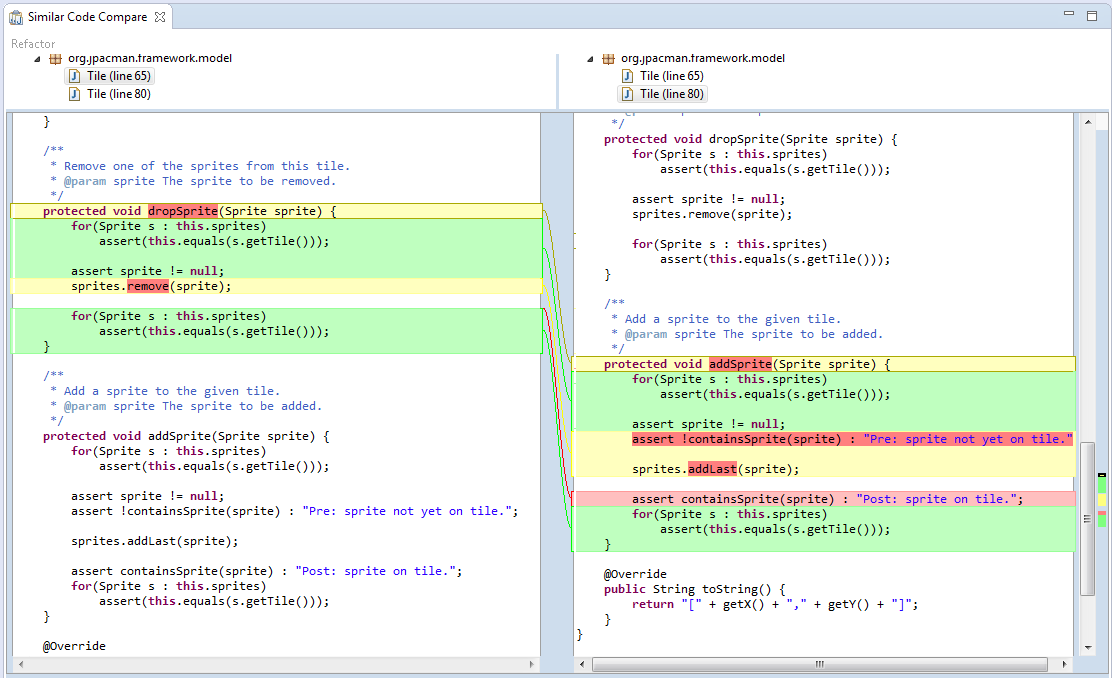
\includegraphics[width=\textwidth]{images/SimilarCode_3.png}
	\caption{\label{SimilarCode3}Détail de l'analyse de code redondant par CodePro}
\end{figure}

\begin{figure}
	\centering
	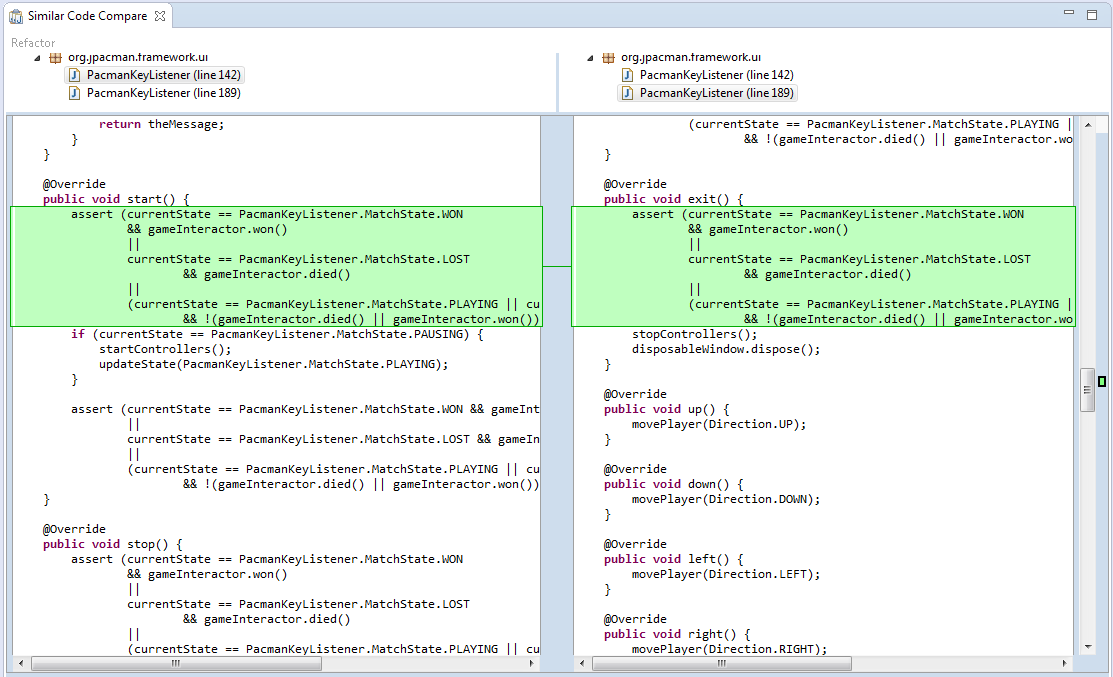
\includegraphics[width=\textwidth]{images/SimilarCode_4.png}
	\caption{\label{SimilarCode4}Détail de l'analyse de code redondant par CodePro}
\end{figure}

\begin{figure}
	\centering
	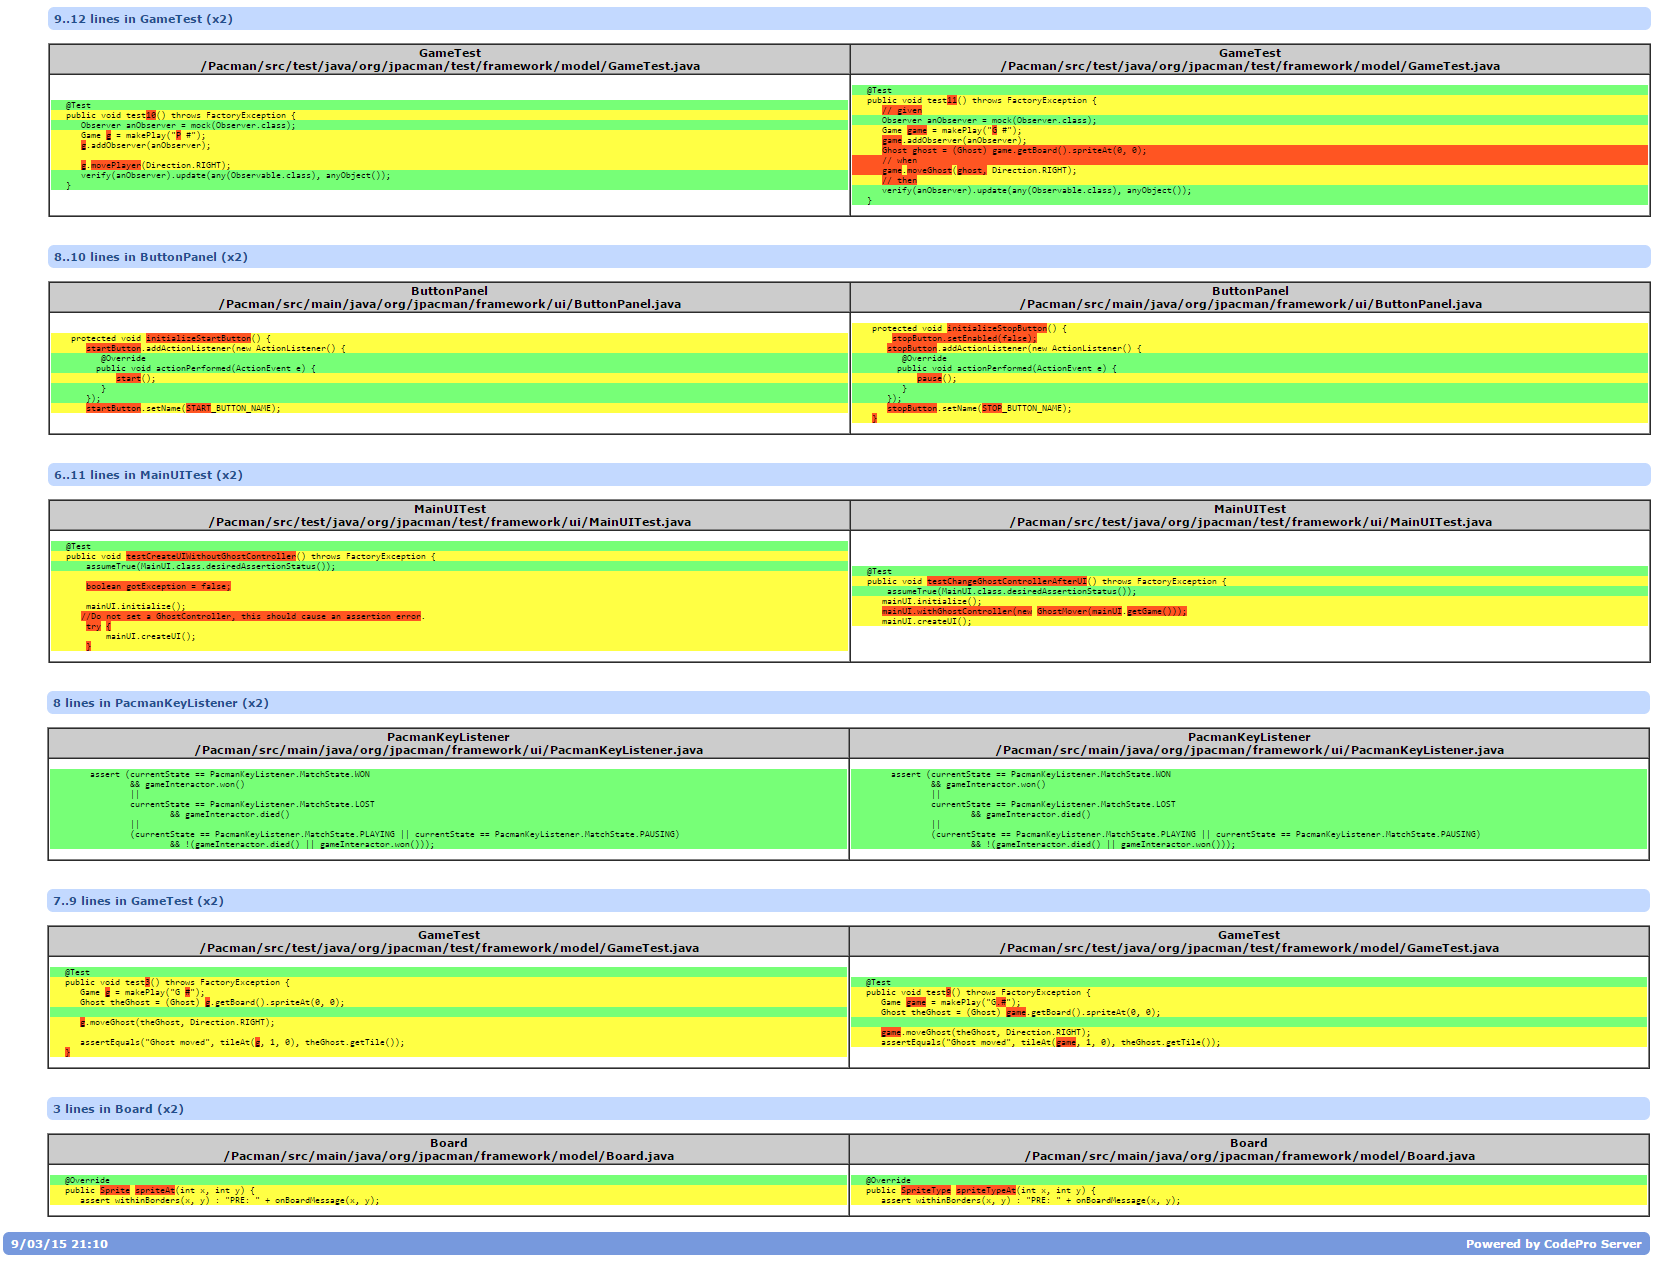
\includegraphics[width=\textwidth]{images/SimilarCode_5.png}
	\caption{\label{SimilarCode5}Détail de l'analyse de code redondant par CodePro (élément dont la visualisation n'est pas possible dans Eclipse)}
\end{figure}

\newpage
\section{Annexe : 2}


\newpage
\bibliographystyle{plain}
\bibliography{reference}

\end{document} 

